\documentclass[12pt]{article}
\usepackage[T1]{fontenc}
\usepackage{lmodern}
\usepackage[a4paper, left=0.7in, right=0.7in, top=0.7in, bottom=0.7in]{geometry}
\usepackage{color} 
\usepackage{hyperref}
\hypersetup{colorlinks=true, linktoc=all, linkcolor=blue, urlcolor=blue}
\usepackage{minted}
\usepackage{underscore}
\usepackage{xcolor}
\usepackage{tcolorbox}
\setlength{\parindent}{0pt}
\setlength{\parskip}{1em}
\usepackage{titlesec}
\titlespacing\section{0pt}{10pt plus 4pt minus 2pt}{-4pt plus 2pt minus 2pt}
\titlespacing\subsection{0pt}{-4pt plus 2pt minus 2pt}{-4pt plus 2pt minus 2pt}
\titlespacing\subsubsection{0pt}{-4pt plus 2pt minus 2pt}{-4pt plus 2pt minus 2pt}
\usepackage[shortlabels]{enumitem}
\setlist[enumerate]{nosep}
\usepackage{amsmath}
\usepackage{float}
\usepackage{graphicx}
\usepackage[space]{grffile}
\usepackage{caption}
\graphicspath{ {./Images2/} }
\begin{document}

\begin{center}
    {\huge Vision Aided Navigation: SLAM}
    \\[1\baselineskip]
    \url{https://github.com/ehud-gordon/VAN_ex}
\end{center}
\tableofcontents
\section{Introduction}
SLAM (Simultaneous Localization and Mapping) builds a map of an unknown environment and localizes an agent's path, revising its estimations as new information is obtained. At each time-step $t$, an agent receives an observation \(o_t\), and simultaneously estimates both its current state $x_t$ and the environment's state $m_t$. Since the estimates use each other, the absolute error accumulates quickly. In order to solve this, global constraints are used to constraint the error, and reduce the drift. The following is an implementation and discussion of a Graph SLAM, using a pose graph with loop closures detection. 

In this implementation, at each time-step the algorithm's front-end receives a new pair of stereo images, and computes the relative motion to the previous pair using PnP. The back-end extracts soft constraints from the data, and incrementally builds a pose graph with edges between keyframes and between loop closures. This graph holds the global constraints of the motion. Finally, the pose graph is optimized, producing a globally consistent path of the agent in the environment. 

The ability to correct initial estimations using only rough observations makes SLAM a useful tool. Visual SLAM turns 2D camera images into an accurate estimation of the 3D world. Since 2D data is simple and cheap to obtain, many industries that require 3D data employ Visual SLAM in their technology. Autonomous vehicles, missiles and vaccum cleaners use SLAM to localize the agent and build a map of the world, allowing accurate navigation obtained from cheap sensors.
\newpage
\section{Overview \& Code}
\subsection{Overview}
Below is an overview of the \href{https://github.com/ehud-gordon/VAN_ex/blob/f82a0a70011392fe57c5ac51b708a5ec6b4a7574/src/stereo_slam.py#L54}{main} method, which consists of a front-end and a back-end. The front-end computes StereoFeatures (2D keypoints + 3D point-cloud) for each two consecutive frames $i$ and $j$, matches between them, and computes the relative pose using PnP. The back-end builds a pose graph from selected keyframes and checks for loop closures. At the end of the drive the pose graph is optimized, and the results are saved.
\begin{tcolorbox} 
\begin{minted}{python}
def main():
    for j in frames[1:]:
        # front-end
        sf_i = get_stereo_features(j-1)
        sf_j = get_stereo_features(j)
        
        matches, sf_i_match, sf_j_match = match_stereo_pairs(sf_i, sf_j)
        pose, inliers = pnp_stereo_ransac(sf_i_match, sf_j_match)
        tracks.add(sf_i, sf_j, inliers)
        
        # back-end
        if is_keyframe(j):
            add_edge_to_pose_graph(last_keyframe, j, tracks)
            check_loop_closures(j)    

    values, covariances = pose_graph.optimize()
    save_results(values, marginals)
\end{minted} 
\end{tcolorbox}
\subsection{Front-end: Triangulation \& PnP}
\href{TODO}{get_stereo_features()} computes StereoFeatures - 2D keypoints matched between the left and right images + a 3D point cloud (pc). \href{TODO}{detectComputeMatch()} finds keypoints using SIFT, matches between them, and a point cloud is generated by \href{TODO}{triangulating} the matching keypoints. Points whose 3D location is unlikely are \href{TODO}{filtered}. A 3D location is unlikely if it lies beyond a certain threshold from the origin. This helps removing outliers and preventing indeterminant linear systems. While this filtering employ specific domain knowledge, I was able to achieve similar results using only sklearn's IsolationForest. However, since it increased the runtime significantly, the simpler approach using threshold values was preferred.
\begin{tcolorbox}
\begin{minted}{python}  
def get_stereo_features(idx):
    left_img, right_img = get_stereo_images(idx)
    keypoints_left, descriptors_left, keypoints_right = \
        detectComputeMatch(left_img, right_img, is_stereo=True)
    
    pc = triangulate(keypoints_left, keypoints_right)
    
    sf = StereoFeatures(idx, keypoints_left, descriptors_left,
                        keypoints_right, pc)
    return filter_stereo_features(sf)
\end{minted}
\end{tcolorbox}
Then, \href{TODO}{match_stereo_pairs()} matches the two cosecutive stereo pairs, and \href{TODO}{pnp_stereo_ransac()} computes a relative pose between them using RANSAC. With RANSAC, in each iteration a pose is computed using only four points, and the subset of inliers for that pose is computed with \href{TODO}{get_pose_inliers()}. The pose with the largest subset of inliers is returned. \\ 
The inputs to \href{TODO}{get_pose_inliers()} are: the pose from the second frame CS to the first frame CS, the matched pixels from the left and right images of frame 1,  and the 3D locations of each point - once from triangulating frame 1's keypoints, and once from triangulating frame 2's keypoints. A point is considered an inlier w.r.t. some pose from CS2 to CS1 if it satisfies both:
\begin{enumerate}
    \item When using the pose to project the 3D location from frame 2 into the pixels of frame 1, it lies near the matching pixels from the left and right images of frame 1.
    \item When using the pose to transform the 3D location from frame 2 into CS 1, the transformed 3D point is near the 3D point received from triangulating frame 1.
\end{enumerate}
Using both conditions to filter outliers was necessary to prevent indeterminant linear systems.
\begin{tcolorbox}
\begin{minted}{python}  
def get_pose_inliers(sf1, sf2, pose_2_to_1, ext_l_to_r, k):
    # check pixel projection errors
    proj_left, proj_right = project(pose_2_to_1, k, sf2.pc, ext_l_to_r)
    error_left = norm(sf1.keypoints_left - proj_left)
    error_right = norm(sf1.keypoints_right - proj_right)
    pixel_inliers = (error_left <= 2) * (error_right <= 2)

    # check point cloud inliers
    pc_2_in_CS_1 = transform_pc_to_world(pose_2_to_1, sf2.pc)
    pc_error = norm(pc_2_in_CS_1 - sf1.pc)
    pc_inliers = pc_error < 3

    inliers = pixel_inliers * pc_inliers
    return inliers
\end{minted}
\end{tcolorbox}
\subsection{Back-end: Pose Graph with Loop Closures}
The computations in the front-end are relative, and don't comply with any global constraints.
Hence, as the drive progresses the estimations acquire drift. In order to capture global constraints, a pose graph is built. A pose graph is a Factor Graph, where the variables are the cameras' poses, and the factors are the relative motion between them, derived from the front-end. In order to reduce the size of the problem, we don't add every frame into the pose graph, but rather select a keyframe every few frames. \\
Factors are probabilistic constraints between the variables. The front-end, however, provides only
improbable measurements. Instead of using some generic assumption about the probability of each motion, another (smaller) factor graph is built, to compute the probability of a motion between two keyframes. I've named this factor graph PixelGraph, since it uses matched pixels along the frames as factors. Specifically, \href{TODO}{PixelGraph().build()} uses the matching tracks (2D keypoints + 3D point cloud), provided by the front-end, to create factors. The variables are the 3D poses of all the cameras between the two keyframes + the 3D locations of the tracks. Since the motion between each frame is small, and therefore relatively constant, a generic probabilistic assumptions can be used for the PixelGraph. Then, the PixelGraph is optimized and the relative covariance between the two keyframes is computed. This also provides Bundle Adjustment. Then, \href{TODO}{pose_graph.add_factor()} adds a factor to the PoseGraph between the new keyframe and the last, using that covariance. 
\begin{tcolorbox}
\begin{minted}{python}  
def add_edge_to_pose_graph(self, frame1, frame2, tracks, frames):
    # Build and optimize PixelGraph
    pixel_graph = PixelGraph().build(frames, poses, tracks)
    values, marginals = pixel_graph.optimize()
    
    # extract relative pose and covariance from factor graph
    pose_from_2_to_1 = get_pose(values, frame1, frame2)
    cov_2_conditional_on_1 = \
        get_conditional_covariance(marginals, frame1, frame2)
    # update distance matrix
    distance_matrix[frame2, frame1] = det(cov_2_conditional_on_1)
    
    # add factor to pose graph
    pose_graph.add_factor(frame1, frame2, pose_from_2_to_1, \
                          cov_2_conditional_on_1)

\end{minted}
\end{tcolorbox}
Next, loop closures between the new keyframe and previous ones are detected. A loop closure (LC) happens when the agent revisits previous locations. Adding LC edges to the pose graph helps constrain the growing covariance.  \href{TODO}{check_loop_closure()} first filters LC candidates by using the Mahalanobis distance. Our assumption is that each two cameras $n$ and $i$ define a Gaussian distribution with covariance $\Sigma_{n|i}$. The Mahalanobis distance between those cameras is: 
\[ ||\Delta c||_{\Sigma} = \Delta c^{T} \Sigma_{n|i} \Delta c \]
where $\Delta c$ is the relative pose. As the computation of $\Sigma_{n|i}$ is expensive, we estimate it by summing over $\Sigma_{j|i}$ for consecutive cameras $i$ and $j$ over the path from $n$ to $i$. Once a LC has formed, several choices for this path can be taken. I've preferred taking the path with the least uncertainty. I've quantified the uncertainty using the determinant of $\Sigma_{j|i}$. However, another sensible choice is simply taking the path with least edges. While the two approaches produce different paths, the resulting $\Sigma_{n|i}$ and $\Delta c$ are equal in practice. Next, further filtering is done by Consensus Match - a PnP pose is computed between the LC candidates, and the percent of inliers is used to estimate the quality of the LC. Higher percent indicates higher probability of a successful LC. For each detected LC, an edge is added to PoseGraph, in a similar fashion as between keyframes.
\begin{tcolorbox}  
\begin{minted}{python}
def check_loop_closures(j):
    sf_j = get_stereo_features(j)
    for k in keyframes[0:-30]:
        # Filter candidates
        path = get_shortest_path(j, k, distance_matrix)
        mahalo_distance = mahalanobis(j, k, poses, covariances, path)
        if mahalo_distance < MAHAL_THRESHOLD:
            # compute relative pose using PnP
            sf_k = get_stereo_features(k)
            pose, inliers, inliers_percent = pnp_stereo(sf_k, sf_j, iters=15)
            if inliers_percent > INLIERS_THRESHOLD:
                # add loop closure edge to pose graph
                tracks = StereoTracksDB().add(sf_k, sf_j, inliers)
                add_edge_to_pose_graph(k, j, tracks)
\end{minted} 
\end{tcolorbox}
Finally, the PoseGraph is optimized and the global poses are computed.

\newpage

\section{Performance Analysis}
The algorithm's performance was evaluated using a drive consisting of 2761 stereo frames from \href{http://www.cvlibs.net/datasets/kitti/setup.php}{kitti setup}. The comparison is done for each keyframe, between the front-end estimations, the final results, and the ground truth provided by kitti. 
\subsection{3D Poses}
Below is a visual demonstration of the path, with ground truth in green. In red are the poses computed by PnP - notice the increasing drift. In orange are the final results of the algorithm, after optimzing the PoseGraph. Notice how close it lies to the ground truth. In blue are the results of optimizing between keyframes using the PixelGraph, but without optizming a PoseGraph. While it doesn't stop the drift, it does provide a more accurate relative motion between keyframes, and hence a more accurate path overall.
\begin{figure}[h]
\centering 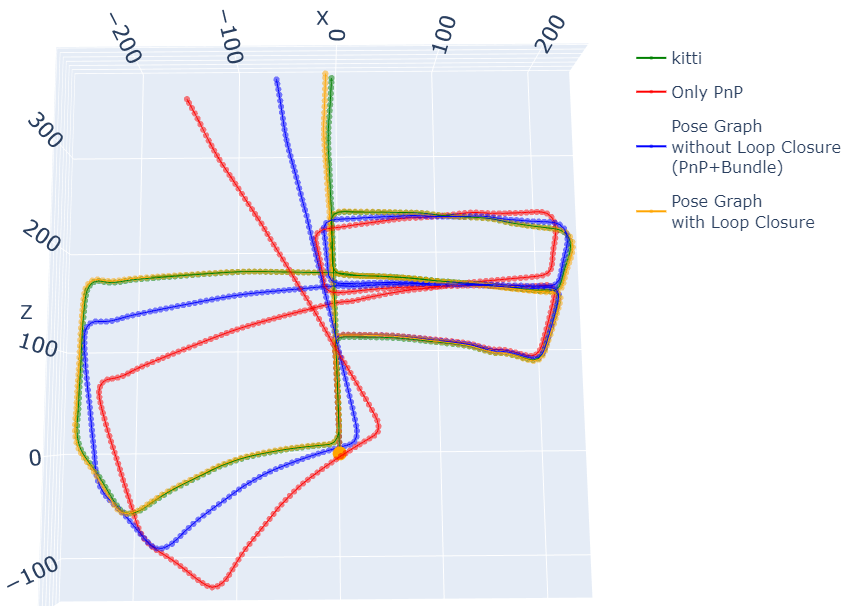
\includegraphics[width=\textwidth]{3D-locations}
\end{figure} \\
Quantitatively, two poses can be compared by looking at their translation and rotation parts. Comparison between translation vectors is done using the Euclidean distance, and rotation matrices can be compared by first finding the relative rotation matrix between them, transforming it into a rotation vector in a Rodrigues representation, and using the L2 norm of that rotation vector. 
\newpage
\subsubsection*{\underline{Relative Error}}
As expected, Bundle Adjustment reduces the relative error. Since the pose graph doesn't change the relative poses significantly, its relative results lie closely to the Bundle ones.\\
The average relative rotation distance, per frame, is 0.03 degrees for PnP, and 0.01 degrees for the PnP+Bundle and the PoseGraph. The average relative translation distance, per frame, is 2 cm for the PnP, and 1cm for the PnP+Bundle and the PoseGraph. The figure below shows the relative rotation error for the three different stages.
\begin{figure}[h]
\centering 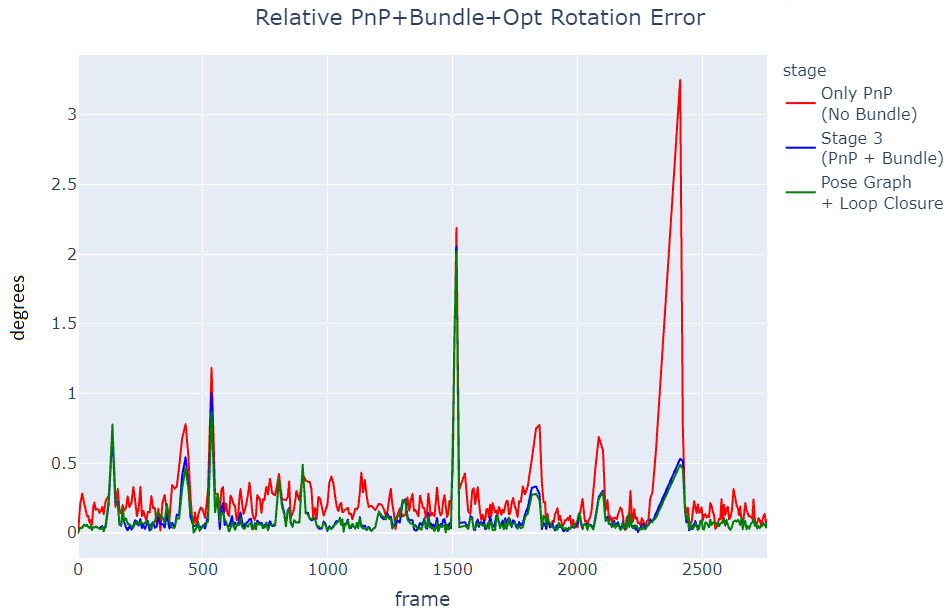
\includegraphics[width=\textwidth]{Relative PnP+Bundle+Opt Rotation Error}
\end{figure} \\
In the figures below, the plot of PnP+Bundle is omitted, since it lies exactly on the PoseGraph plot. Axes labels are on the right. 
\begin{figure}[H]
\centering 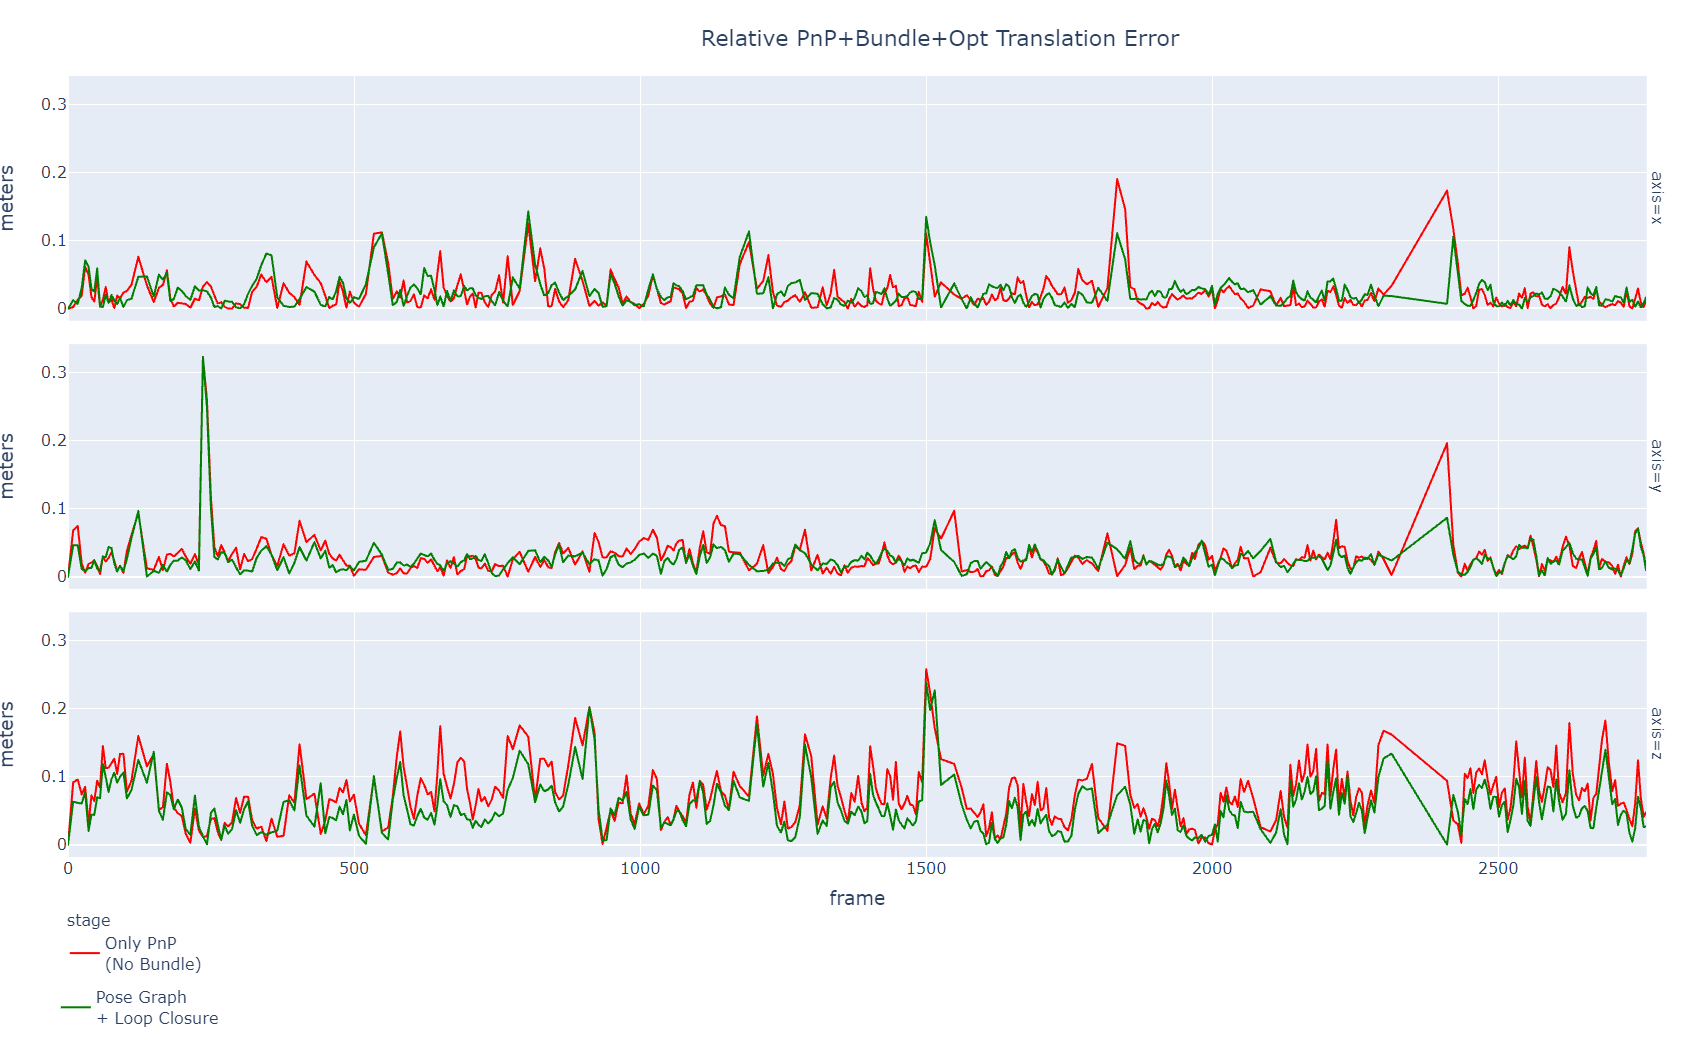
\includegraphics[width=\textwidth]{Relative PnP+Opt Translation Error}
\end{figure} 
The figure above shows the relative translation error per axis. It can be seen that the error is largest in the $z$-axis. This might be due to the range of the 3D points. While in the $x$ and $y$ axes the points are at most $30$ meters away, in the $z$-axis they can be $200$ meters far. \\
Below is the Euclidean distance for the relative translation vectors.
\begin{figure}[H]
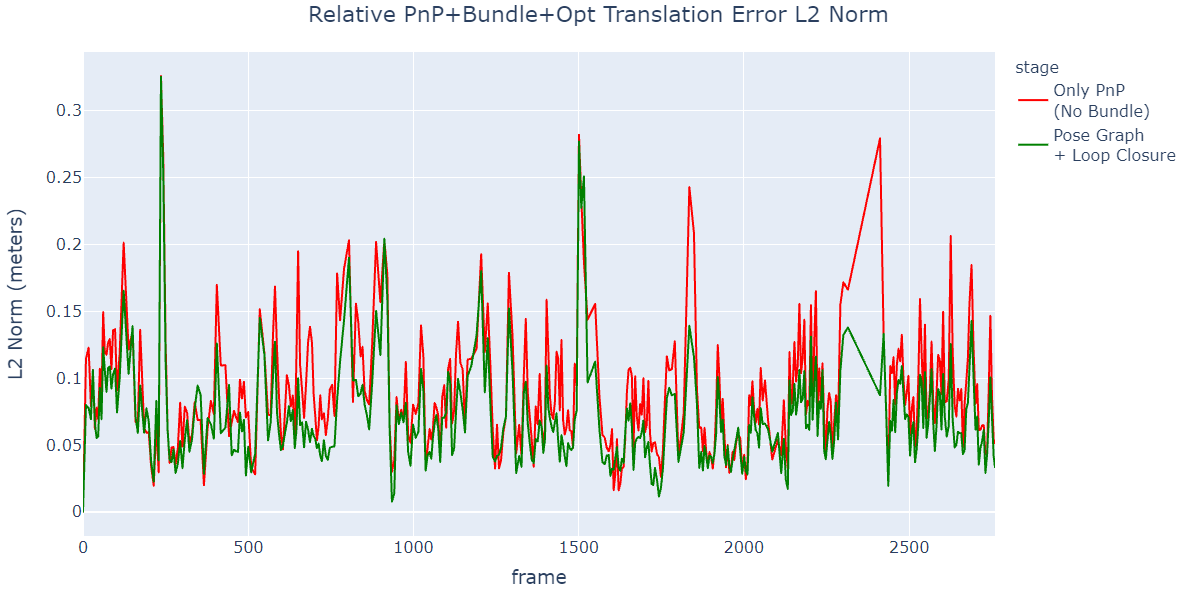
\includegraphics[width=\textwidth, height=0.4\textheight]{Relative PnP+Bundle+Opt Translation Error L2 Norm2}
\end{figure} 
As expcted, when using Bundle Adjustment the translation error is lower as well. 
\newpage
\subsubsection*{\underline{Absolute Error}}
Next, the poses w.r.t. to the start of the drive are compared. This shows that using global constraints (LC detection) improves the overall path. The average absolute rotation error, per frame, is 2.3 degrees for PnP, 0.8 degrees for PnP+Bundle, and 0.1 degrees for PoseGraph. The average absolute translation error, per frame, is 9.1 meters for PnP, 3.1 meters for PnP+Bundle, and 0.4 meters for the PoseGraph. Below are the absolute rotation erros for the three stages.
\begin{figure}[h]
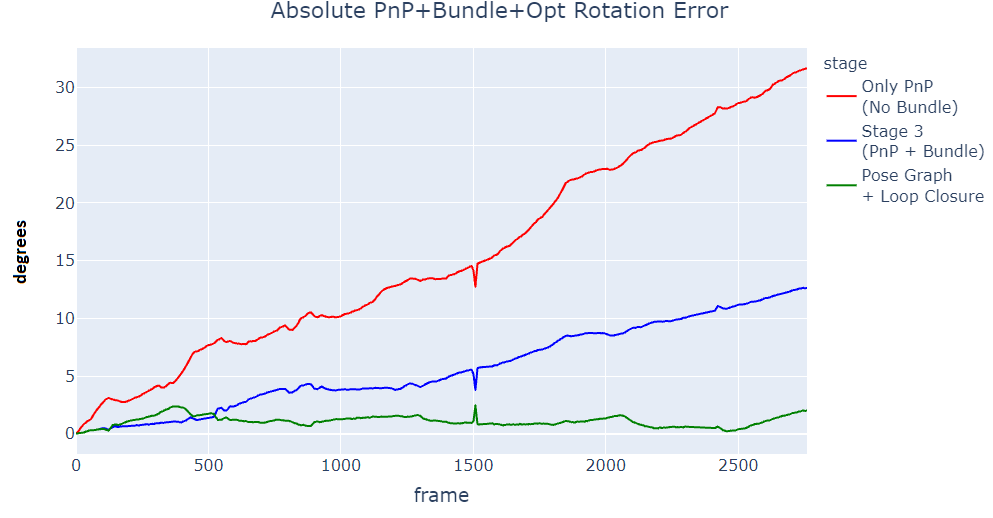
\includegraphics[width=\textwidth]{Absolute PnP+Bundle+Opt Rotation Error}
\end{figure} \\
It's remarkable how the the error increases for both the PnP and PnP+Bundle as the drive progress, but the PoseGraph is able to constrain the error. 
\begin{figure}[h]
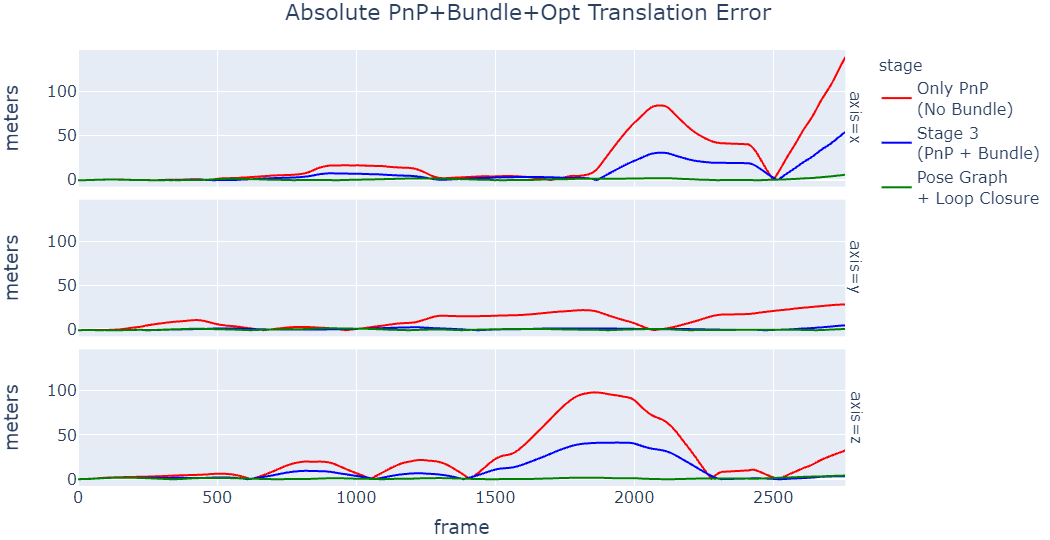
\includegraphics[width=\textwidth]{Absolute PnP+Bundle+Opt Translation Error}
\end{figure} \\
The figure above shows the absolute translation error for each axis. It seems that the error in the $y$ axis is the smallest, but this is probably due to the fact that the difference between the two most distant points along the $y$-axis is only 15 meters, while it's around 400 meters for the $x$ and $z$ axes.
\\ Below is the Euclidean distance for the absolute translation vectors.
\begin{figure}[H]
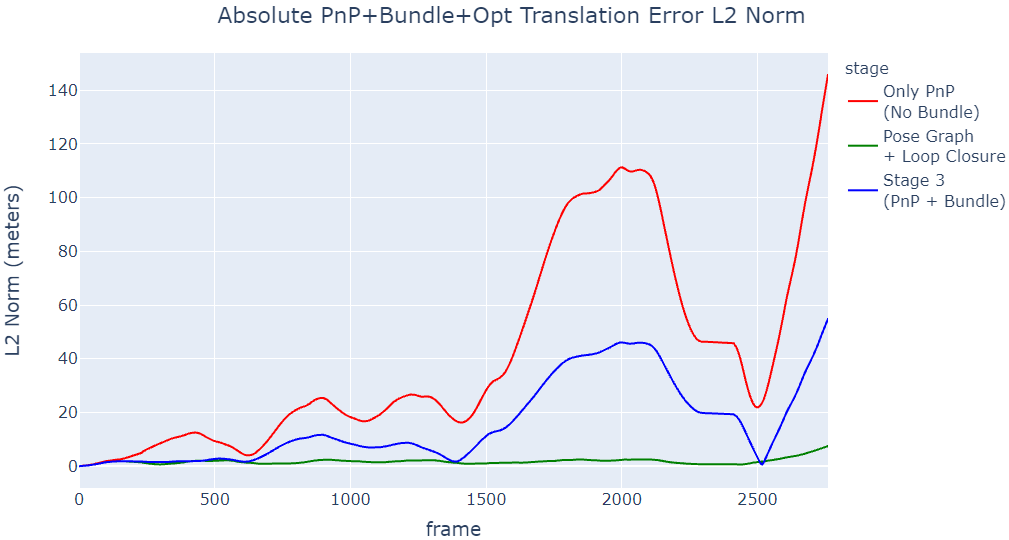
\includegraphics[width=\textwidth]{Absolute PnP+Bundle+Opt Translation Error L2 Norm}
\end{figure}

Due to the randomness in the directon of the drift error, at one point the PnP+Bundle estimation is closer to the ground truth than all other estimations. In general, however, the PoseGraph+LC is significantly closer. 
\subsubsection*{\underline{Is the Pose Graph just a poser?}}
An interesting question is whether we can achieve similar results with less effort. One idea I've tested is using loop closures without a pose graph. Specifically, after detecting loop closures, we can compute a camera's absolute pose by composing the relative poses we've computed along the shortest path to the start. In the figures below, I've called this "Stage 3 with LC". While the pose graph performs better, this approach comes close.
The per-frame average absolute rotation errors are 0.8, 0.19 and 0.16 degrees for Stage3 (PnP+Bundle), Stage3+LC, and the Pose Graph, respectively. Similarly, The per-frame average absolute translation errors are 3.1, 0.68 and 0.41 meters. 
\begin{figure}[H]
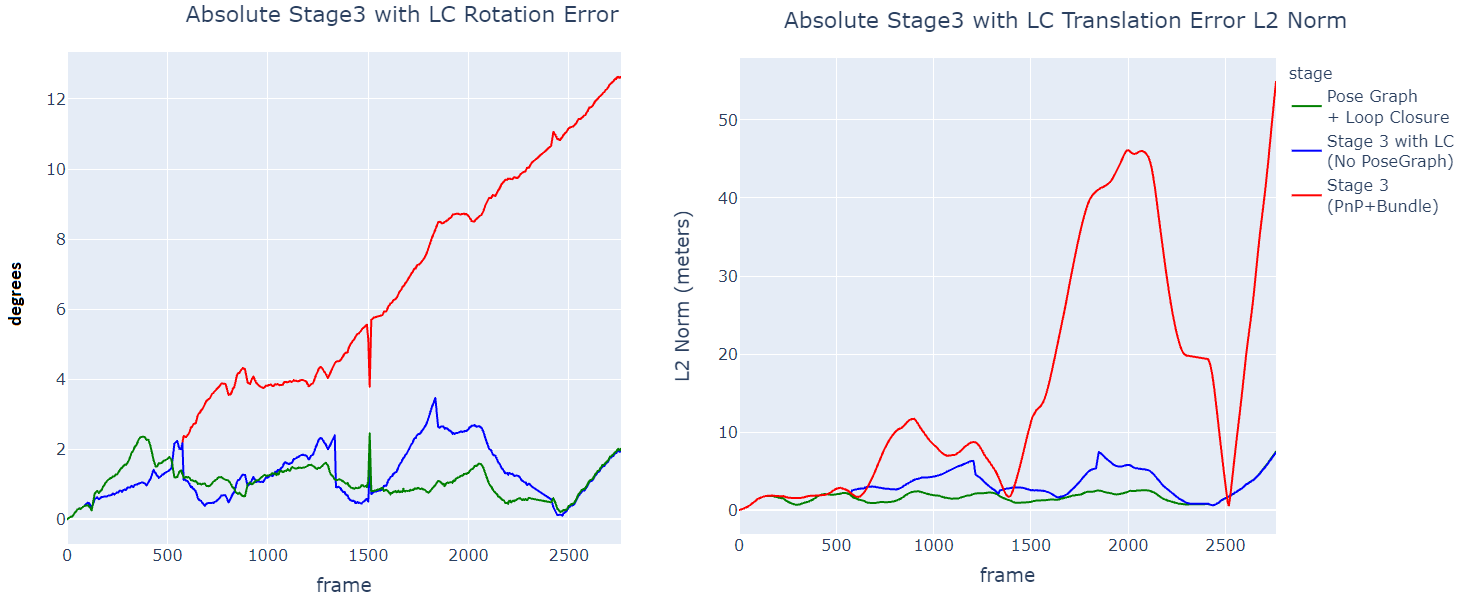
\includegraphics[width=\textwidth]{Stage3 With LC}
\end{figure}

\newpage
\subsection{Features}
The front-end uses 2D keypoints detection and matching when computing poses. 
For each stereo pair, we first find matching keypoints between the left and right images, and then use those to match to the following stereo pairs. Out of those, only some will be inliers for the computed PnP pose. The figures below shows these values. I've also added the number of consecutive matching keypoints for the loop closure edges, demonstrating that they're a harder match. 
\begin{figure}[H]
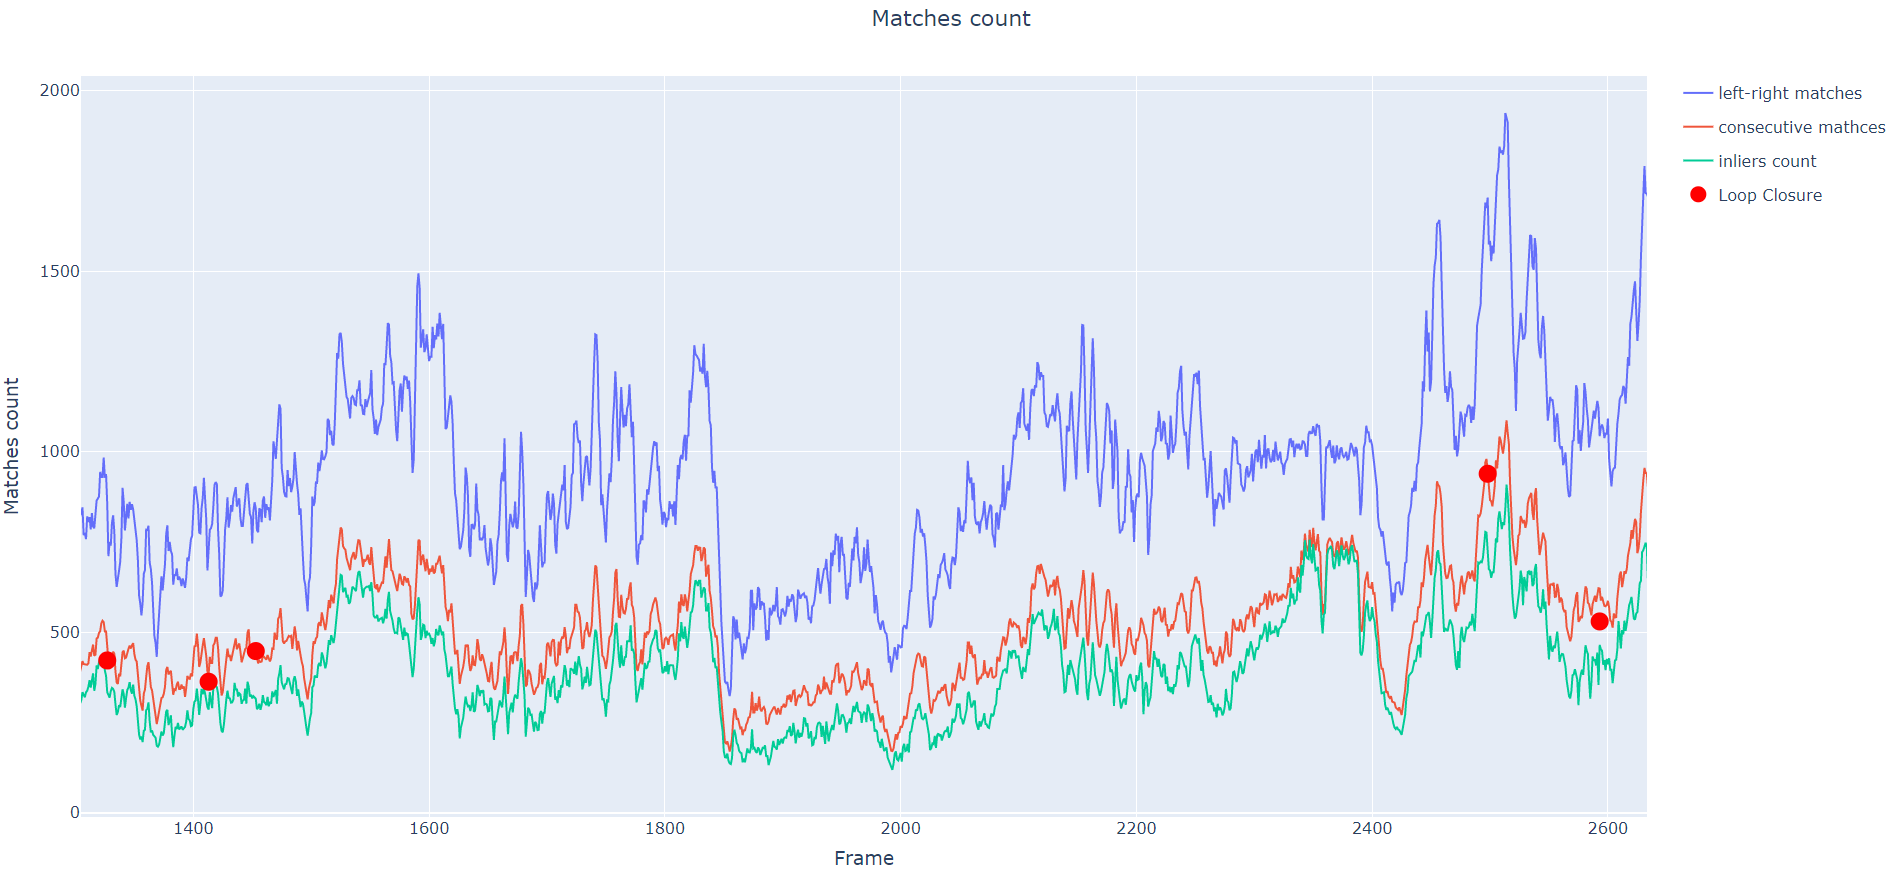
\includegraphics[width=\textwidth]{matches count}
\end{figure}

\begin{figure}[H]
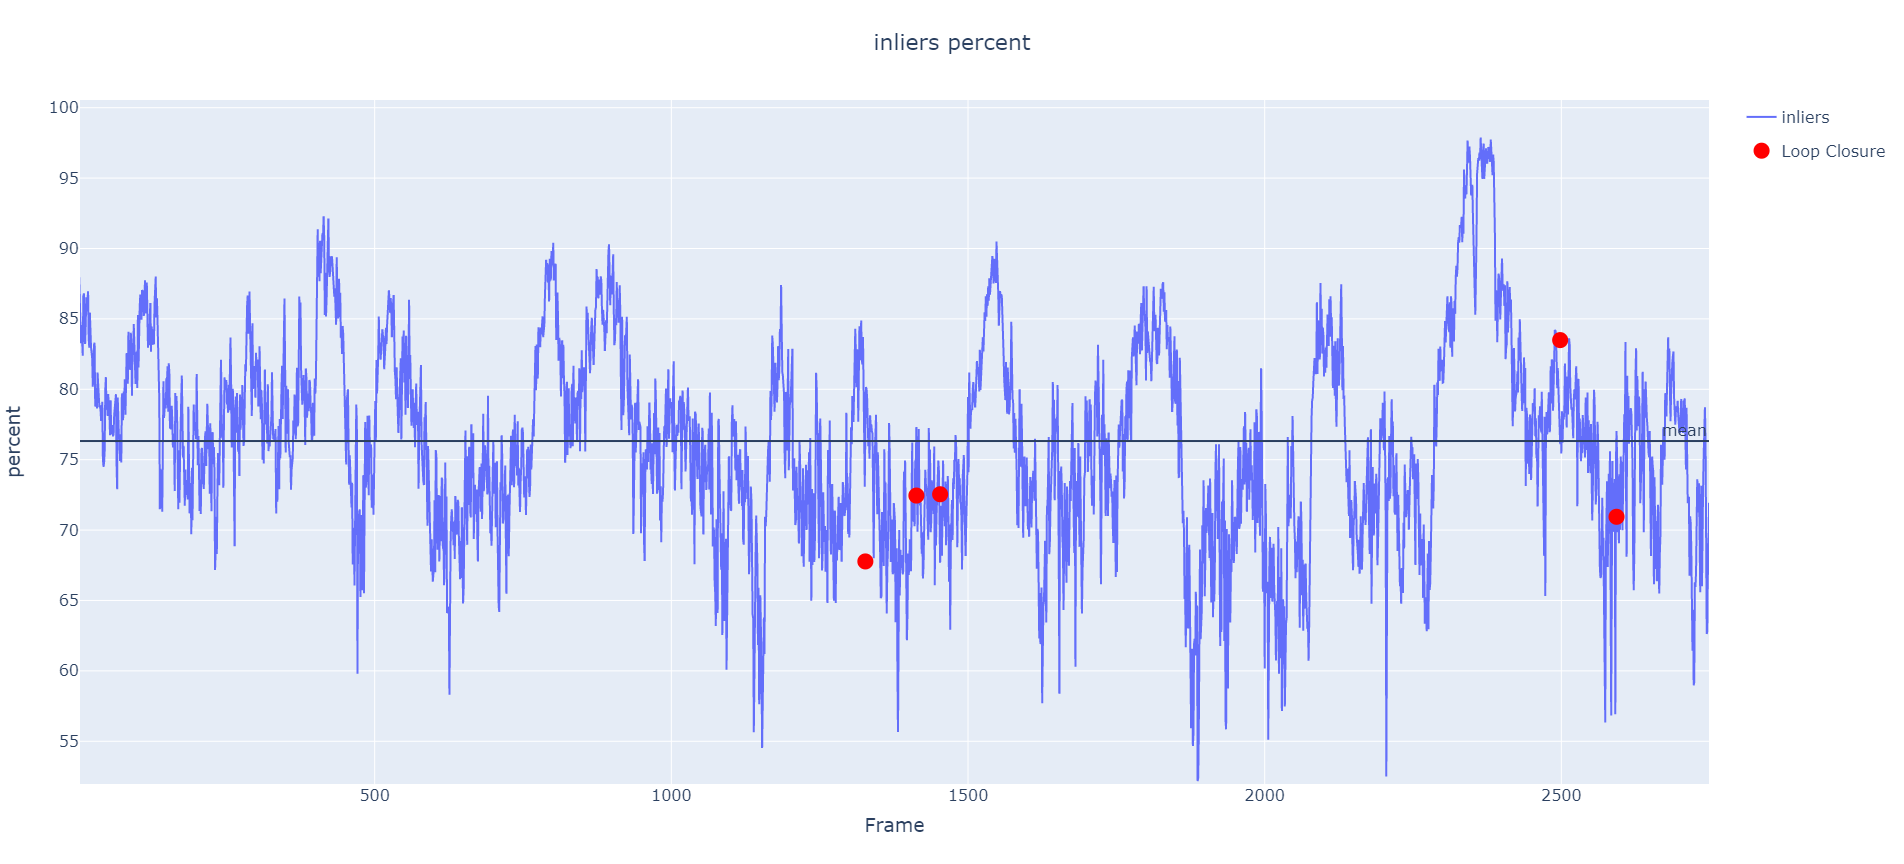
\includegraphics[width=\textwidth]{inliers percent}
\end{figure}
The PnP inliers are used as tracks when performing Bundle Adjustment. The longer the the track length, the better the constraints for the Bundle, and therefore a more accurate poses will results. 1.5 million tracks were detected, 560 keypoints on average per frame. The mean track length was 3.4. Below I've included a hisogram of the track lengths, as well as a plot of the connectivity - the number of tracks outgoing to the next frame (400 on average).

\newpage
\begin{figure}[H]
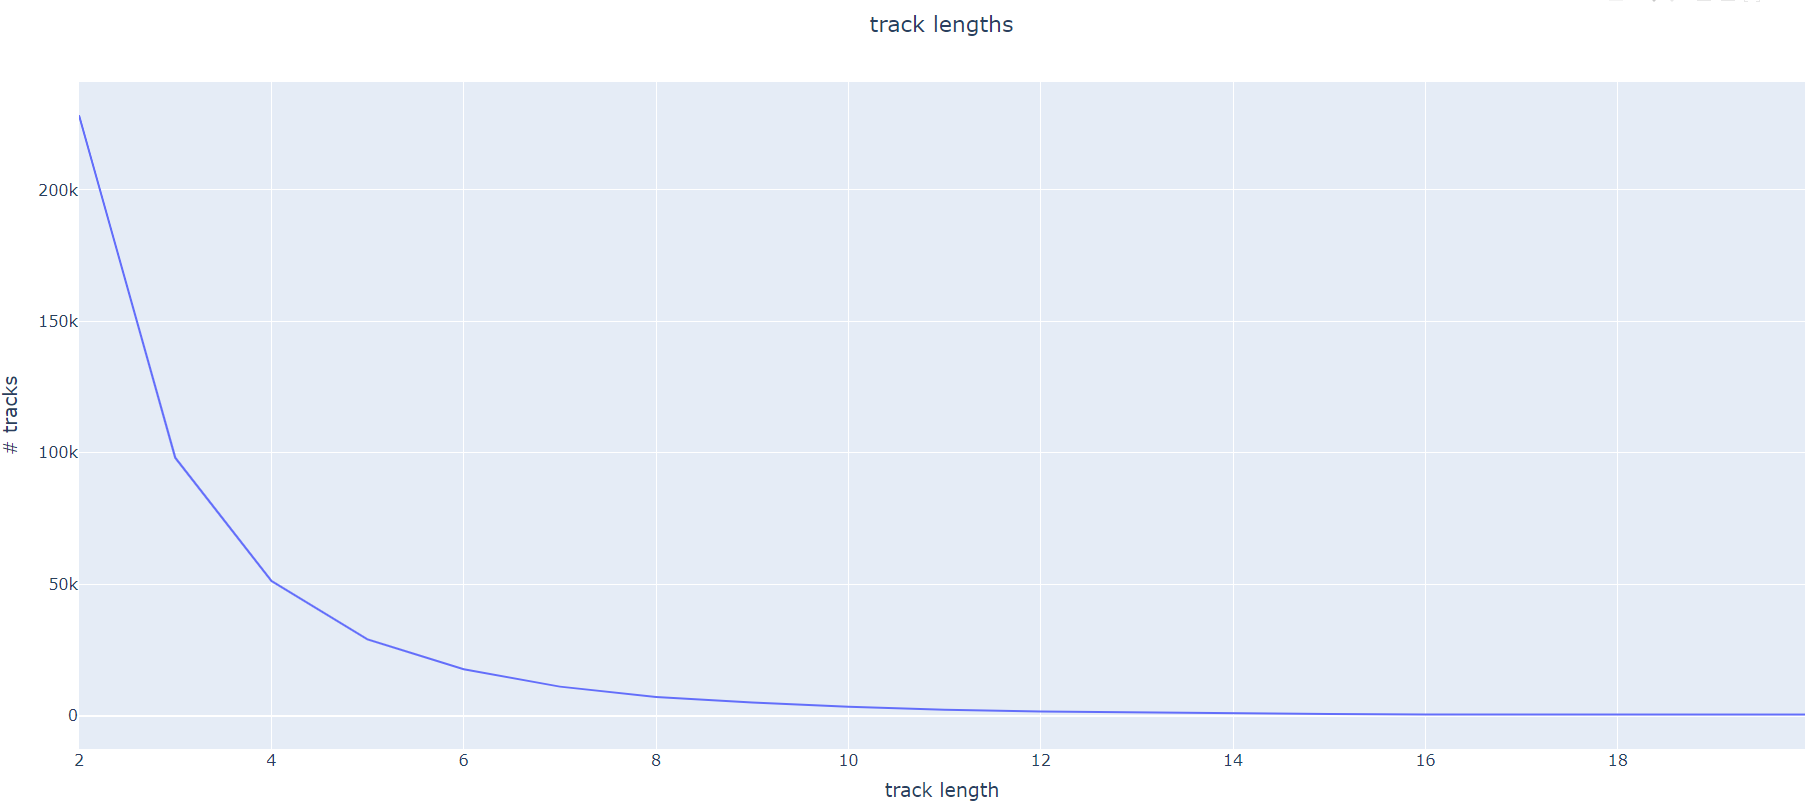
\includegraphics[width=\textwidth, height=0.25\textheight]{track lengths}
\end{figure}

\begin{figure}[H]
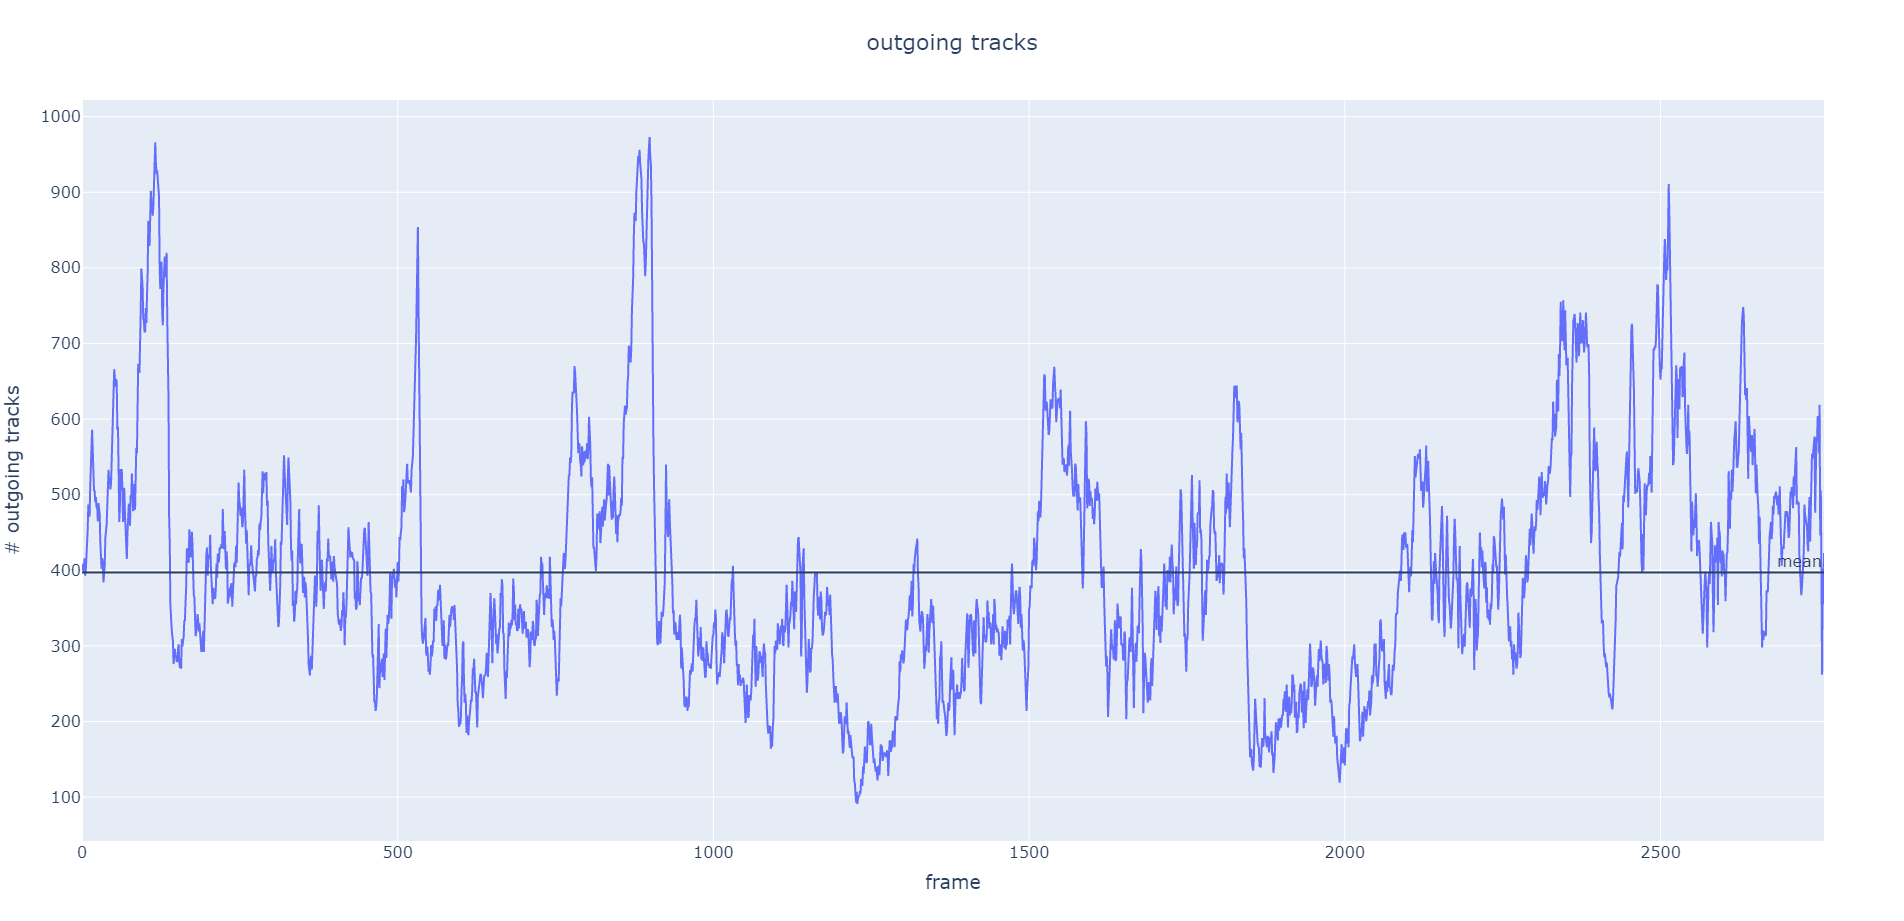
\includegraphics[width=\textwidth, height=0.25\textheight]{outgoing tracks}
\end{figure}

When performing Bundle Adjustment, the 3D locations of the tracks are part of the variables. The triangulation from the first frame along the track is used as initial estimate. Below are the projection erros of those locations onto the frames along the track length, as a function of the distance from the reference. We compare between the median projection and median factor errors of the initial estimate (in blue) and the resulting locations after Bundle Adjustment (in red).
\begin{figure}[H]
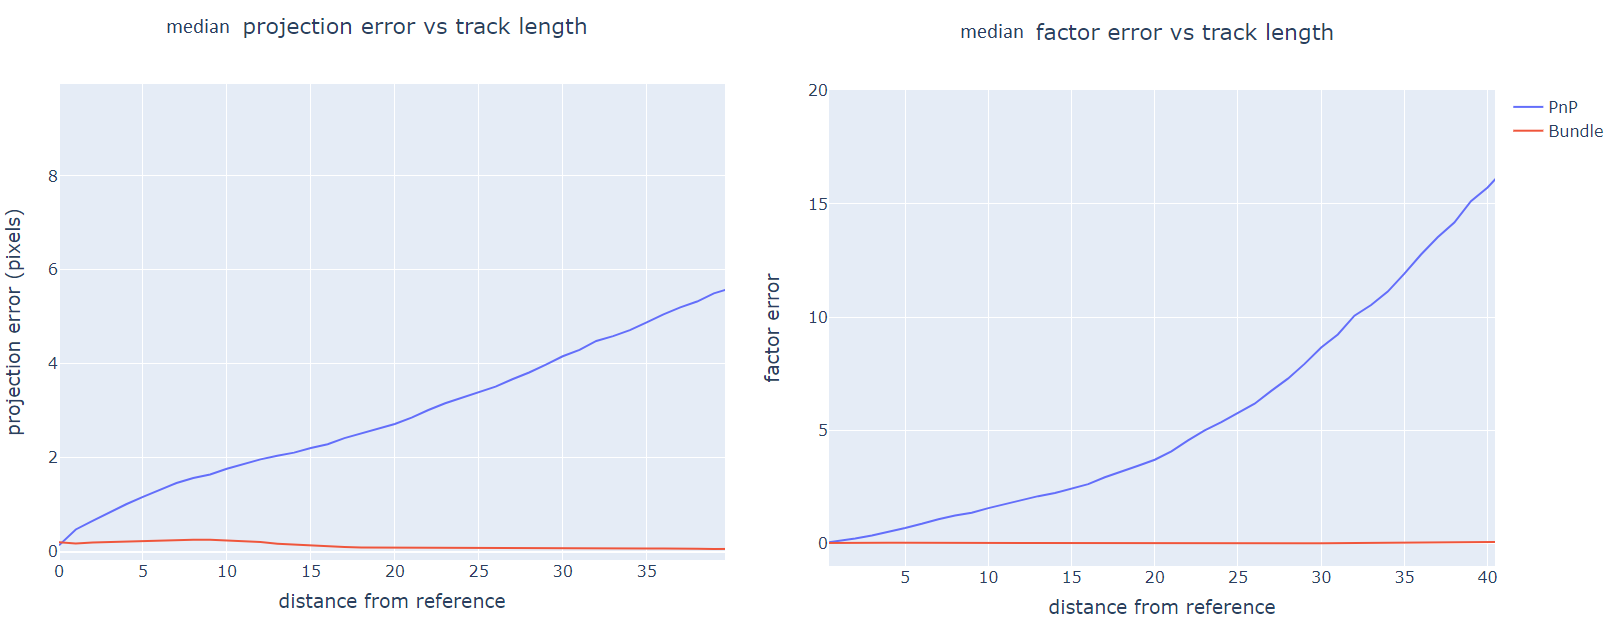
\includegraphics[width=\textwidth]{proj fact error}
\end{figure}

\newpage
\subsection{Uncertainty}
In addition to providing more consistent results, using a pose graph with global constraints also reduces our uncertainty about the cameras' locations. We quantify the uncertainty using the determinant of the (estimated) relative covariance matrix. That is, for camera $i$, we look at $\Sigma_{i|0}$, a $(6,6)$ matrix, where the upper-left (3,3) block relates to the yaw-pitch-roll rotation parameters, and the lower-right (3,3) block to the x,y,z translation parameters. The determinant of each of these blocks can be used to quantify the uncertainty we have.
\begin{figure}[H]
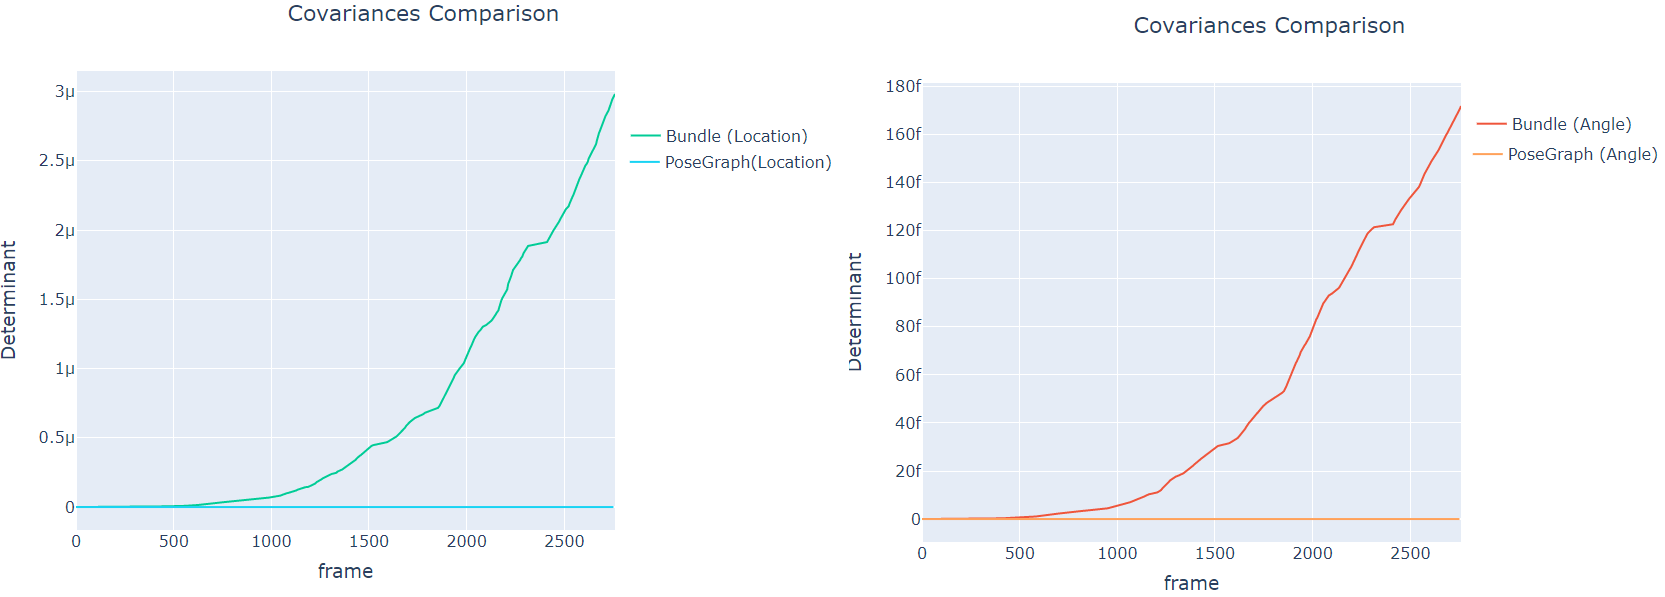
\includegraphics[width=\textwidth]{determinant angle location}
\end{figure}
\subsection*{Mahalanobis distance}
Below I've added the graph I've used to determine the Mahalanobis distance threshold when filtering for LC candidates. For each frame, the Mahal distance to all possible previous candidates is computed, and the closest three are plotted. This shows nicely the loop closure regions. 
\begin{figure}[H]
\caption*{Mahalanobis Distance}
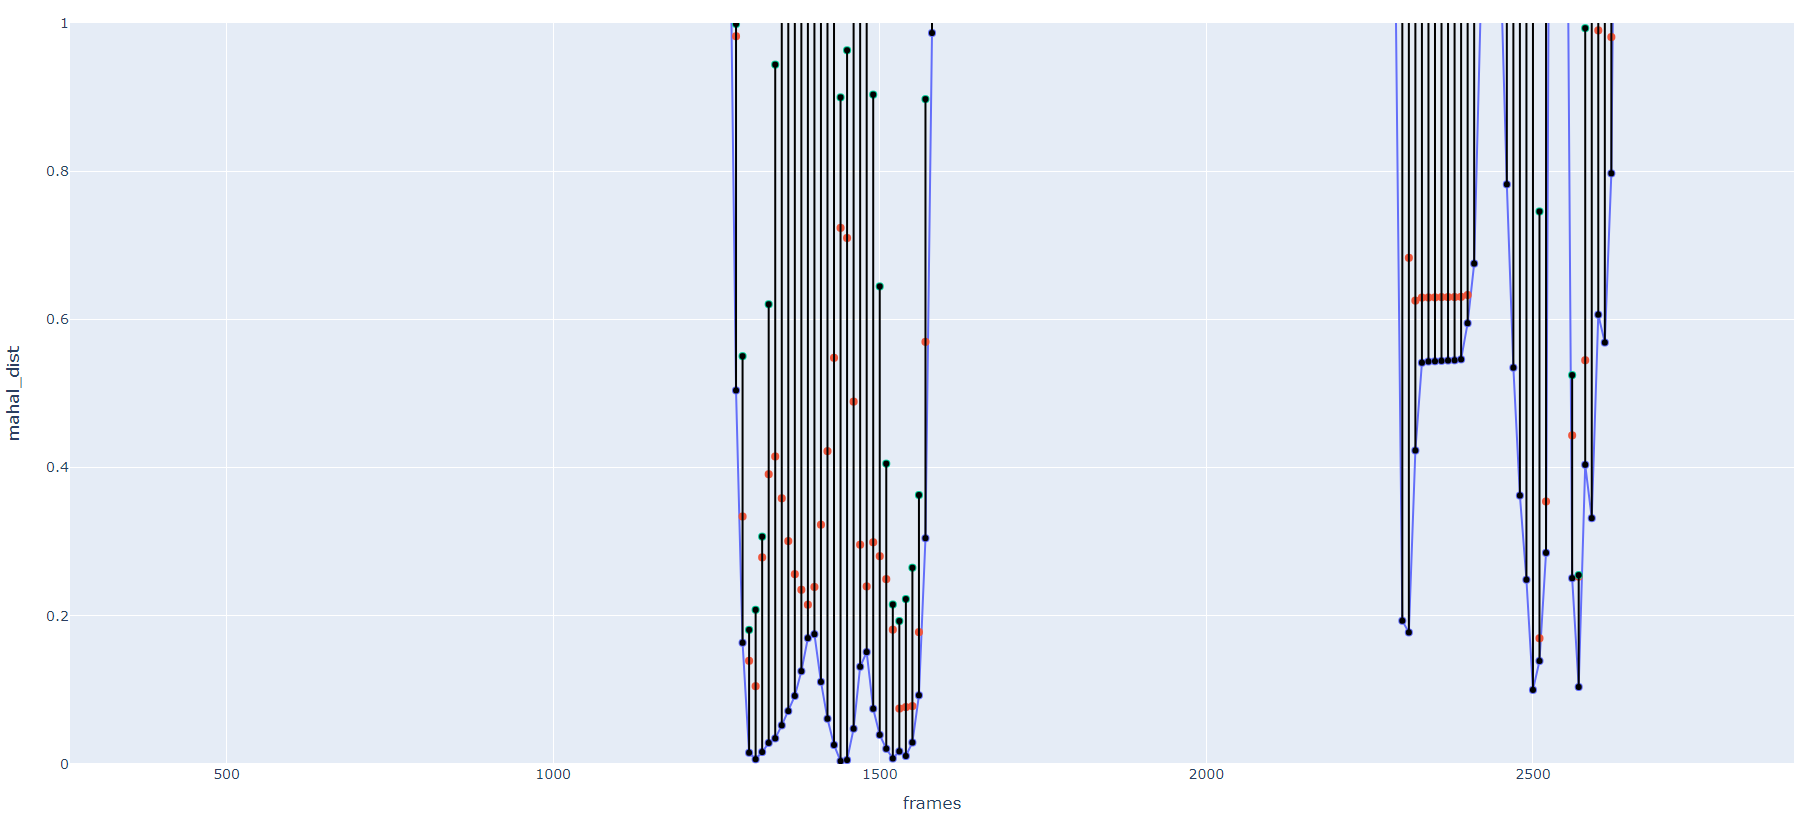
\includegraphics[width=\textwidth]{mahal dist}
\end{figure}
\newpage
\section{Conclusion}
In this report I've discussed the approach of using pose graph with loop closures detection in order to perform Visual SLAM. I've evaluated it using real-world data, and showed that it was able to constrain the accumulative drift, and reduce both the relative and absolute error of simpler appraoches. 

There are several shortcomings to my analysis:
  First, the test data isn't diverse enough. It contained no occlusions, frame drops or agressive motions, and presented many long and unique loop closure events. In order to truly assess the efficacy of this approach, it must be evaluted on a more challenging dataset.
  The short track lengths (3.4 on average) are also problematic, since they cause the Bundle Adjustment results to be suboptimal. Better keypoint detection and outlier rejection could produce more accurate poses, and reflecting more accurately the effect of using a pose graph or loop closures. I've tried using different keypoints algorithms such as STAR and BRIEF, but no improvement was visible. 
  Another concern is the necessity of using a pose graph. Under the section "Is the Pose Graph just a poser?" I've shown that a significant improvement can be made using only loop closures, without any pose graph.

The use of loop closures requires several conditions. First, the agent must revisit past locations, a requirement that isn't met by many outdoor agents. Further, as the drive progresses, the cost of checking for LC increases. Additionally, elaborate methods must be implemented in order to prevent conflicting loop closures constraints. All of the above limit the availability of LC detection. 

Finally, while using a pose graph with loop closures helped reduce the absolute error, it almost didn't reduce the relative error. Whereas Bundle Adjustment was able to fix the initial estimations made by the PnP, the constraints introduced by the pose graph were too global to impact lower-resolution details such as relative poses. Perhaps adding some pixel constraints into the pose graph will help reduce the relative error even further.  

There are many avenues for further work. Other methods of creating global constraints can be used - GPS, for example, is another cheap sensor whose data can be added to the pose graph. Different choices can be made for the front-end - such as using more cameras when performing PnP, or using nonlinear triangulation. Different choices can be made for the back-end as well - solving constraints can be achieved using a Kalman Filter or a Particle Filter. \\ Another possible idea is using loop closure events for self-supervised learning. A neural network can be trained to guess relative poses, and loop closure can be used to inject supervised data into the system.

\end{document}